\documentclass{article}
\usepackage{amsthm}
\usepackage{amsmath}
\usepackage{amssymb}
\usepackage{amsfonts}
\usepackage{graphicx}
\usepackage{wrapfig}
\usepackage{tabu}
\usepackage{hyperref}
\usepackage{booktabs}
\usepackage{listings}
\graphicspath{ {./Images/} }

\makeatletter
\def\lecture{\@ifnextchar[{\@lectureWith}{\@lectureWithout}}
\def\@lectureWith[#1]{\medbreak\refstepcounter{section}%
	\renewcommand{\leftmark}{Lecture \thesection}
	\noindent{\addcontentsline{toc}{section}{Lecture \thesection: #1\@addpunct{.}}%
		\sectionfont Lecture \thesection. #1\@addpunct{.}}\medbreak}
\def\@lectureWithout{\medbreak\refstepcounter{section}%
	\renewcommand{\leftmark}{Lecture \thesection}
	\noindent{\addcontentsline{toc}{section}{Lecture \thesection.}%
		\sectionfont Lecture \thesection.}\medbreak}
\makeatother

\newcommand{\n}{\newline}

\title{CMSC 660 HW III}
\date{9/19/18}
\author{Joe Asercion}
\begin{document}
	\maketitle

	Note: I unfortunately ran out of time to finish this HW (was just one of those weeks).  The current problem parts are missing in their entirety and have been deleted for the sake of brevity: 1.d, 2.a, 2.g, 2.h, 3.b.\n
	
	\section{Chapter 4, Problem 11}
	Given the following information:
	\begin{itemize}
		\item $\frac{1}{2}\delta_{x}^{2}u=f(x)$ for $0<x<1$ 
		\item Boundary Conditions: $u(0)=u(1)=0$
		\item Discretized interval: $[0,1]$ in a uniform grid of points $x_{j}=j\Delta x$ with $n\Delta x=1$
		\item  $n-1$ unknowns $U_{j}$ are approximations to $u(x_{j}),\text{ }j=1,...,n-1$
		\item Second order approximation: $\frac{1}{2}\frac{1}{\Delta x^{2}}(U_{j+1}-2U_{j}+U_{j-1})=f(x_j)=F_j$\\
		\item These linear equations can be written as $AU=F$
	\end{itemize}
	\subsection{a. Calculation}
	Check that there are $n-1$ distinct eigenvectors of $A$ having the form $r_{kj}=\sin(k\pi x_{j})$ where $r_{kj}$ is the $j$ component of the eigenvector $r_{k}$.
	\subsubsection{Answer}
	
	We are given the expression $AU=F$ and are told the form of both $F$ and $U$.  Therefore we can calculate the form the matrix $A$ must be in: \n
	
	\begin{align*}
		U&=\begin{bmatrix}
			0\\
			U_{1}\\
			U_{2}\\
			U_{3}\\
			...\\
			U_{n-1}\\
			0
			\end{bmatrix}\\
		F_j&=\frac{1}{2}\frac{1}{\Delta x^{2}}(U_{j+1}-2U_{j}+U_{j-1})=f(x_j)\\
		\therefore A&=\frac{1}{2}\frac{1}{\Delta x^{2}}\begin{bmatrix}
		-2 & 1 & 0 & 0 & 0 & ... & 0\\
		1 & -2 & 1 & 0 & 0 & 0 & ...\\
		0 & 1 & -2 & 1 & 0 & 0 & ... \\
		0 & 0 & 1 & -2 & 1 & 0 & ... \\
		... & ... & ... & ... & ... & ... & ... \\
		... & ... & ... & 0 & 1 & -2 & 1 \\
		0 & ... & ... & ... & 0 & 1 & -2 
		\end{bmatrix}
	\end{align*}
	Where $A$ has dimensions of $(n-1)\times (n-1)$.  \n
	
	Let $R_{k}$ be the $kth$ vector consisting of elements $r_{kj}=sin(k\pi x_{j})$.  If $R_{k}$ is an eigenvector of matrix $A$ then it satisfies
	
	\begin{align*}
		AR_{k}=\lambda_{k}R_{k}
	\end{align*}  
	
	Where $\lambda_{k}$ is the eigenvalue associated with the $k^{th}$ eigenvector.  Starting with the $k=1$ case we can plug in values and expand this expression:
	
	\begin{align*}
	 \frac{1}{2}\frac{1}{\Delta x^{2}}\begin{bmatrix}
	-2 & 1 & 0 & 0 & 0 & ... & 0\\
	1 & -2 & 1 & 0 & 0 & 0 & ...\\
	0 & 1 & -2 & 1 & 0 & 0 & ... \\
	0 & 0 & 1 & -2 & 1 & 0 & ... \\
	... & ... & ... & ... & ... & ... & ... \\
	... & ... & ... & 0 & 1 & -2 & 1 \\
	0 & ... & ... & ... & 0 & 1 & -2 
	\end{bmatrix}
	\begin{bmatrix}
	\sin(\pi x_{1}) \\
	\sin(\pi x_{1+1})\\
	\sin(\pi x_{1+2})\\
	\sin(\pi x_{1+3})\\
	...\\
	\sin(\pi x_{n-1})
	\end{bmatrix}=\lambda_{1}
	\begin{bmatrix}
	\sin(\pi x_{1}) \\
	\sin(\pi x_{1+1})\\
	\sin(\pi x_{1+2})\\
	\sin(\pi x_{1+3})\\
	...\\
	\sin(\pi x_{n-1})
	\end{bmatrix}
	\end{align*}
	
	Noting that $r_{k,j+1}=\sin(k\pi(x+\Delta x))$, and that $n\Delta x=1$, we can rewrite the above expression as 
	
	\begin{align*}
	&\frac{1}{2}\frac{1}{\Delta x^{2}}\begin{bmatrix}
	-2 & 1 & 0 & 0 & 0 & ... & 0\\
	1 & -2 & 1 & 0 & 0 & 0 & ...\\
	0 & 1 & -2 & 1 & 0 & 0 & ... \\
	0 & 0 & 1 & -2 & 1 & 0 & ... \\
	... & ... & ... & ... & ... & ... & ... \\
	... & ... & ... & 0 & 1 & -2 & 1 \\
	0 & ... & ... & ... & 0 & 1 & -2 
	\end{bmatrix}
	\begin{bmatrix}
	\sin(\pi x_{1}) \\
	\sin(\pi (x_{1}+\Delta x))\\
	\sin(\pi (x_{1}+2\Delta x))\\
	\sin(\pi (x_{1}+3\Delta x))\\
	...\\
	\sin(\pi(x_{1}+(n-3)\Delta x))\\
	\sin(\pi (x_{1}+(n-2)\Delta x))
	\end{bmatrix}=\lambda_{1}
	\begin{bmatrix}
	\sin(\pi x_{1}) \\
	\sin(\pi (x_{1}+\Delta x))\\
	\sin(\pi (x_{1}+2\Delta x))\\
	\sin(\pi (x_{1}+3\Delta x))\\
	...\\
	\sin(\pi(x_{1}+(n-3)\Delta x))\\
	\sin(\pi (x_{1}+(n-2)\Delta x))
	\end{bmatrix}\\
	\end{align*}
	
	Which gives equations of the form 
	
	\begin{align*}
	&\frac{1}{2}\frac{1}{\Delta x^{2}}(-2\sin(\pi x_{1})+\sin(\pi(x_{1}+\Delta x)))=\lambda_{1}\sin(\pi x_{1})\\
	&\frac{1}{2}\frac{1}{\Delta x^{2}}(\sin(\pi x_{1})-2\sin(\pi (x_{1}+\Delta x))+\sin(\pi(x_{1}+2\Delta x)))=\lambda_{1}\sin(\pi x_{1}+\Delta x)\\
	&\frac{1}{2}\frac{1}{\Delta x^{2}}(\sin(\pi x_{1}+\Delta x)-2\sin(\pi x_{1}+2\Delta x)+\sin(\pi(x_{1}+3\Delta x)))=\lambda_{1}\sin(\pi (x_{1}+2\Delta x))\\
	&...\\
	&\frac{1}{2}\frac{1}{\Delta x^{2}}(\sin(\pi(x_{1}+(n-4)\Delta x))-2\sin(\pi(x_{1}+(n-3)\Delta x))+\sin(\pi(x_{1}+(n-2)\Delta x)))\\&=\lambda_{1}\sin(\pi(x_{1}+(n-3)\Delta x))\\
	&\frac{1}{2}\frac{1}{\Delta x^{2}}(\sin(\pi(x_{1}+(n-3)\Delta x))-2\sin(\pi(x_{1}+(n-2)\Delta x)))\\&=\lambda_{1}\sin(\pi(x_{1}+(n-2)\Delta x))\\
	\end{align*}
	
	Using the given fact that $n\Delta x=1$, the generated equations can be simplified:
	
	\begin{align*}
		&\frac{1}{2}\frac{1}{\Delta x^{2}}(-2\sin(\pi x_{1})+\sin(\pi(x_{1}+\Delta x)))=\lambda_{1}\sin(\pi x_{1})\\
		&\frac{1}{2}\frac{1}{\Delta x^{2}}(\sin(\pi x_{1})-2\sin(\pi (x_{1}+\Delta x))+\sin(\pi(x_{1}+2\Delta x)))=\lambda_{1}\sin(\pi x_{1}+\Delta x)\\
		&\frac{1}{2}\frac{1}{\Delta x^{2}}(\sin(\pi x_{1}+\Delta x)-2\sin(\pi x_{1}+2\Delta x)+\sin(\pi(x_{1}+3\Delta x)))=\lambda_{1}\sin(\pi (x_{1}+2\Delta x))\\
		&...\\
		&\frac{1}{2}\frac{1}{\Delta x^{2}}(\sin(\pi(x_{1}+1-4\Delta x))-2\sin(\pi(x_{1}+1-3\Delta x))+\sin(\pi(x_{1}+1-2\Delta x)))\\&=\lambda_{1}\sin(\pi(x_{1}+1-3\Delta x))\\
		&\frac{1}{2}\frac{1}{\Delta x^{2}}(\sin(\pi(x_{1}+1-3\Delta x))-2\sin(\pi(x_{1}+1-2\Delta x)))\\&=\lambda_{1}\sin(\pi(x_{1}+1-2\Delta x))\\
	\end{align*}
	
	Applying $x_{j}=j\Delta x$...
	
	\begin{align*}
		&\frac{1}{2}\frac{1}{\Delta x^{2}}(-2\sin(\pi \Delta x)+\sin(2\pi\Delta x))=\lambda_{1}\sin(\pi\Delta x)\\
		&\frac{1}{2}\frac{1}{\Delta x^{2}}(\sin(\pi \Delta x)-2\sin(2\pi\Delta x)+\sin(3\pi\Delta x))=\lambda_{1}\sin(2\pi\Delta x)\\
		&\frac{1}{2}\frac{1}{\Delta x^{2}}(\sin(2\pi\Delta x)-2\sin(3\pi\Delta x)+\sin(4\pi\Delta x))=\lambda_{1}\sin(3\pi\Delta x)\\
		&...\\
		&\frac{1}{2}\frac{1}{\Delta x^{2}}(\sin(\pi(1-3\Delta x))-2\sin(\pi(1-2\Delta x))+\sin(\pi(1-\Delta x)))=\lambda_{1}\sin(\pi(1-2\Delta x))\\
		&\frac{1}{2}\frac{1}{\Delta x^{2}}(\sin(\pi(1-2\Delta x))-2\sin(\pi(1-\Delta x)))=\lambda_{1}\sin(\pi(1-\Delta x))\\
	\end{align*}
	
	Applying a bit of algebra and the identities of trigonometric functions allows us to isolate the $\lambda_{1}$ eigenvalue:
	
	\begin{align*}
		\frac{\cos(\pi\Delta x)-1}{\Delta x^2}=\lambda_{1}\\
	\end{align*}
	
	Generalizing this for all $k$ yields:
	
	\begin{equation}
		\frac{\cos(k\pi\Delta x)-1}{\Delta x^2}=\lambda_{k}
	\end{equation}
	
	Since (1) is a scalar value solely dependent on the step size $\Delta x$ and the index $k$, it shows that the vector $R_{k}$ is in fact an eigenvector of matrix $A$.  As noted in \cite{BG}(pg. 77), the $(n-1)\times(n-1)$ matrix $A$ may have up to $n-1$ eigenvectors.  We see that (1) implies that iterating the value of $k$ generates a distinct eigenvalue, therefore the set of eigenvectors associated with the eigenvalues defined by (1) are linearly independent and form a basis for $\mathbb{C}^{n-1}$ \cite{BG}(pg. 77).  Therefore, there must be $n-1$ eigenvectors of $A$ in the form of $R_{k}$.

	\subsection{b. Calculation}
	Use te eigenvalue information from part (a) to show that $||A^{-1}||\rightarrow\frac{2}{\pi^{2}}$ as $n\rightarrow\infty$ and $\kappa(A)=\mathcal{O}(n^{2})$ as $n\rightarrow\infty$.  (Use Euclidian Norms). 
	
	\subsubsection{Answer}	
	
	 From 4.2.7 Theorem 1 \cite{BG}(pg. 82), if a matrix is self-adjoint the Rayleigh Quotient of an eigenvector is its corresponding eigenvalue.  Plugging in the values found in part a we obtain:
	
	\begin{align*}
		Q(x)=\lambda_{k}&=\frac{R_{k}^{*}AR_{k}}{R_{k}^{*}R_{k}}\\
		\frac{\cos(k\pi\Delta x)-1}{\Delta x^{2}}&=\frac{(\sin(k\pi x_{j}))^{*} A\sin(k\pi x_{j})}{(\sin(k\pi x_{j}))^{*}\sin(k\pi x_{j})}
	\end{align*}
	
	From the definition of the Euclidian Norm of a matrix \cite{BG}(pg. 76), we see that the maximum of Rayleigh Quotient is the Euclidean Norm of the matrix $A$ squared.  i.e.
	
	\begin{equation}
		||A||_{l^{2}}=max\Big(\frac{\cos(k\pi\Delta x)-1}{\Delta x^{2}}\Big)=max\Big(n^{2}(\cos(k\pi\frac{1}{n})-1)\Big)
	\end{equation}

	Taking the limit of (2) as $n\rightarrow\infty$ yields
	
	\begin{align*}
		\lim_{n\rightarrow\infty}n^{2}(\cos(k\pi\frac{1}{n})-1)=-\frac{k^2\pi^2}{2}
	\end{align*}
	
	To find the norm of $||A^{-1}||$ we need to invert this expression:
	
	\begin{equation}
		||A^{-1}||_{l^{2}}=\frac{2}{\pi^{2}}
	\end{equation}
	
	Informally, $\kappa(A)$ is on the order of $\mathcal{O}(n^{2})$ due to the condition number of an eigenvalue problems's dependence on the the norm of $\Delta A$\cite{BG}(pg. 92).  In (2) the dominant term as $n\rightarrow\infty$ will the the leading $n^{2}$ term.  Therefore the overall condition number of the Eigenvalue problem will be on the order of $n^{2}$.
	
	\subsection{c. Calculation}
		Given:
		\begin{itemize}
			\item $\tilde{U_{j}}=u(x_j)$, where $u(x)$ is the exact but unknown solution to the BVP
			\item $R=A\tilde{U}-F$ is defined to be the residual
		\end{itemize}
		Show that if $u(x)$ is smooth then the residual satisfies $||R||=\mathcal{O}(\Delta x^{2})=\mathcal{O}(\frac{1}{n^{2}})$
	\subsubsection{Answer}
		From the statement of the problem we know $F=AU$.  Therefore, we can rewrite the residual as 
		
		\begin{align*}
			R=A\tilde{U}-AU
		\end{align*}
		
		Therefore,
		
		\begin{align*}
			||R||=||A\tilde{U}-AU||\leq||A\tilde{U}||-||AU||\leq||A|| ||\tilde{U}||-||A|| ||U|| \text{\cite{BG} (pg. 74)}
		\end{align*}
		
		From part B we know the norm of $||A||$, therefore
		
		\begin{align*}
			||R||&=\frac{\cos(k\pi\Delta x)-1}{\Delta x^{2}}||\tilde{U}||-\frac{\cos(k\pi\Delta x)-1}{\Delta x^{2}}||U||\\
			&=\frac{\cos(k\pi\Delta x)-1}{\Delta x^{2}}(||\tilde{U}||-||U||)\\
			&=\frac{\cos(k\pi\Delta x)-1}{\Delta x^{2}}(||\Delta x\sum_{k=1}^{n}\tilde{U_{j}^{2}}||-||\Delta x\sum_{k=1}^{n}U_{j}^{2}||)\\
			||R||&=\frac{\cos(k\pi\Delta x)-1}{\Delta x}(||\sum_{k=1}^{n}\tilde{U_{j}^{2}}||-||\sum_{k=1}^{n}U_{j}^{2}||)
		\end{align*}
	\newpage
	\subsection{f. MATLAB}
		Write a program in MATLAB to solve $AU=F$ for the second order method.
		\subsubsection{Answer}
		\begin{lstlisting}
		%*****************************
		% CMSC660 HW3 Problem 1f
		% Joe Asercion
		%***************************** 
		
		% Set iteration step size
		delta_x=.001;
		
		% Total number of steps
		n=(1/delta_x);
		
		% Vector to hold F(x) function values
		F=ones(n-1,1);
		
		% Constant for Eigenvector F(x) case
		k=1;
		
		% Populate F(x) vector
		for j = 1:(n-1)
		% Define function to populate F(x) with here:
		F(j)=sin(k*pi*(j*delta_x));
		end
		
		% 'A' Transformation Matrix
		A = (1/2)*(1/(delta_x)^2)*gallery('tridiag',n-1,1,-2,1);
		
		% Solution for AU=F using MATLAB backslash operator
		U = A\F;
		
		% Vector consisting of steps for plot
		X = 0+delta_x:delta_x:1-delta_x;
		
		% Plot delta_x vs U(x)
		scatter(X,U)
		\end{lstlisting}
		This scatter plot shows the approximation generated by the program when $\Delta x=0.001$ and $f(x)=sin(\pi x))$
		
		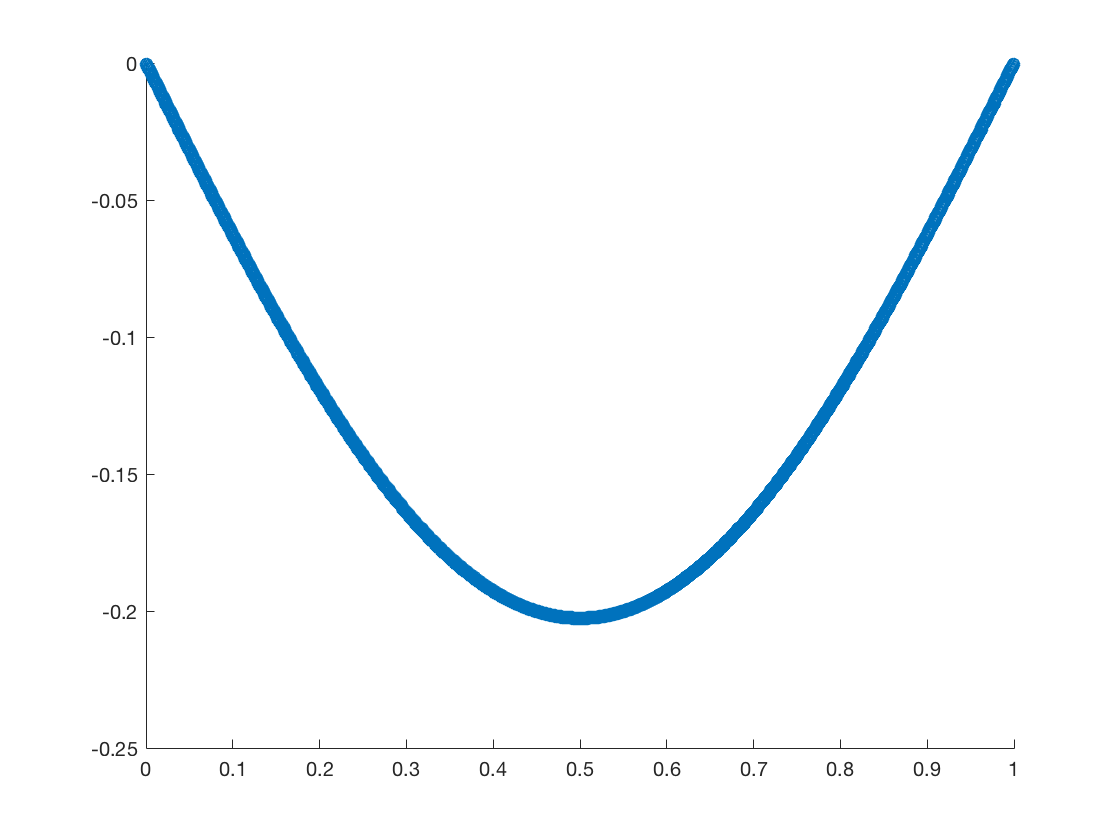
\includegraphics[width=\textwidth]{scatter.png} 

	\section{Chapter 4, Problem 12}
		\subsection{b. Calculation}
		Use matrix norms and the fact that $||B^{k}||\leq||B||^{k}$ to show that the matrix exponential $e^{B}=\sum_{k=0}^{\infty}\frac{1}{k!}B^{K}$ converges.
		\subsubsection{Answer}
		
		Using the given fact that $||B^{k}||\leq||B||^{k}$, we can state that, for each individual term in sum, 
		
		\begin{equation}
			||\frac{B^{k}}{k!}||\leq\frac{||B||^{k}}{k!}
		\end{equation}
		
		From the definition of the matrix norm \cite{BG}(pg. 76), it can be noted that $||B||$ is the sharp constant in the inequality above.  Therefore, norm of each individual term of the matrix exponential sum is upper bounded by the norm of the matrix itself. \n
		
		Because the norm of B, $||B||$, is a scalar function we can note that $\sum_{k=0}^{\infty}\frac{||B||^k}{k!}$ is in the form of the Exponential Series, which is known to be convergent.  Due to (4),
		
		\begin{align*}
			\sum_{k=0}^{\infty}||\frac{B^k}{k!}||\leq\sum_{k=0}^{\infty}\frac{||B||^k}{k!}
		\end{align*} 
		
		Therefore, by the Direct Comparison convergence test\cite{ComTest} we can state that $\sum_{k=0}^{\infty}||\frac{B^k}{k!}||$ must converge as well.  Because the norm of a matrix is, by definition, the largest amount it can stretch a vector\cite{BG}(pg. 76), 
		
		\begin{align*}
			\sum_{k=0}^{\infty}\frac{1}{k!}B^{K}\leq\sum_{k=0}^{\infty}||\frac{B^k}{k!}
		\end{align*}
		
		By the Direct Comparison test once again we can state that $\sum_{k=0}^{\infty}\frac{1}{k!}B^{k}$ must converge.
		
		\subsection{c. Calculation}
		Show that the fundamental solution is given by $S(t)=e^{tA}$.
		\subsubsection{Answer}
		
		\textbf{First Condition:} Is $\frac{d}{dt}S(t)=S(t)A$?\n
		
		Expressing $S(t)$ as an infinite sum,
		
		\begin{align*}
			S(t)&=\sum_{k=0}^{\infty}\frac{1}{k!}(tA)^{k}=1+tA+\frac{(tA)^2}{2}+\frac{(tA)^3}{6}+\frac{(tA)^4}{24}+.... \\
			\therefore \frac{d}{dt}(S(t))&=\frac{d}{dt}(\sum_{k=0}^{\infty}\frac{(tA)^{k}}{k!})=\sum_{k=1}^{\infty}\frac{k(t^{k-1})A^k}{k!}=A+tA^2+\frac{t^2A^3}{2}+\frac{t^3A^4}{6}+\frac{t^4A^5}{24}+...\\
			\therefore \frac{d}{dt}S(t)&=S(t)A
		\end{align*}
		
		\textbf{Second Condition:} Is $S(0)=I$?\n
		
		Again expressing $S(t)$ as an infinite sum,
		
		\begin{align*}
			S(0)&=\sum_{k=0}^{\infty}\frac{(0A)^k}{k!}=\sum_{k=0}^{\infty}\frac{\mathbf{0}^k}{k!}
		\end{align*}
		
		Where $\mathbf{0}$ is a zero matrix with the dimensions of $A$.  $\mathbf{0}^n=I$ for $n=0$ and $\mathbf{0}^n=\mathbf{0}$ for $n\neq0$.  Therefore $S(0)=I$.
		
		
		\subsection{d. Calculation}
		Show that $e^{tA}=Re^{t\Lambda}L$ and that $e^{t\Lambda}$ is the obvious diagonal matrix
		\subsubsection{Answer}
		
		Let $A=R\Lambda L$.  Then
		
		\begin{align*}
			e^{tA}&=\sum_{k=0}^{\infty}\frac{(tA)^k}{k!}\\
			&=\sum_{k=0}^{\infty}\frac{(tR\Lambda L)^k}{k!}=\sum_{k=0}^{\infty}\frac{t^k(R\Lambda L)^k}{k!}
		\end{align*}
		
		Examining the $(R\Lambda L)^k$ term,
		
		\begin{align*}
			(R\lambda L)^{k}=(R\lambda L)(R\lambda L)(R\lambda L)....
		\end{align*}
		
		However, $L=R^{-1}$.  Therefore, the only two $R$ and $L$ matrices that persist at the end of the product will be the $R$ at the head of the term and the $L$ at the tail.  The sum can thusly be rewritten as
		
		\begin{align*}
			e^{tA}=\sum_{k=0}^{\infty}\frac{t^{k}R\Lambda^{k}L}{k!}
		\end{align*}
		
		Since $R$ and $L$ are no longer subject to the index $k$ (as they appear once in each term of the sum), they can be pulled out of the summation and the expression can be simplified:
		
		\begin{align*}
			e^{tA}&=\sum_{k=0}^{\infty}\frac{t^{k}R\Lambda^{k}L}{k!}\\
			&=R(\sum_{k=0}^{\infty}\frac{t^{k}\Lambda^{k}}{k!})L\\
			&=Re^{t\Lambda}L
		\end{align*}
		
		$e^{t\Lambda}$ is the obvious diagonal matrix for $e^{tA}$ as it simply takes the matrix exponential of the scaled $\Lambda$.  The original $\Lambda$ matrix is only being modified along the diagonal, since nothing is being added to it, and the scaled eigenvalues in the $e^{t\Lambda}$ matrix still correspond with the $R$ and $L$ eigenvectors, as shown above.
		
		\newpage
		\subsection{e. MATLAB}
		Calculate the eigenvalues and right eigenvector matrix of A using the Matlab eig(A) function.  Print $r_{k},Ar_{k},\lambda_{k}r_{k}$ and $||\lambda_{k}r_{k}-Ar_{k}||$  
		\subsubsection{Answer}
		\begin{lstlisting}
		%*****************************
		% CMSC660 HW3 Problem 2e
		% Joe Asercion
		%***************************** 
		
		% Set Markov chain transition matrix constants
		lambda = 1;
		mu = 4;
		
		% Time constant
		t = 1;
		
		% Iterations
		n = 4;
		k = 20;
		
		% Preallocate matrices to store the eigenvalues and eigenvectors returned 
		% by eig[A]
		R = zeros(n);
		Lam = zeros(n);
		
		% Build the MCT matrix.  Call a test tridiag matrix of size n-1 and change
		% elements [1, 1] and [n, n] to their correct values.
		A = gallery('tridiag',n,mu,-(lambda+mu),lambda);
		A(1, 1) = -lambda;
		A(n, n) = -mu;
		
		% Convert sparse matrix A to a full matrix so that eig can be called
		A = full(A);
		
		% Call eig to calculate eigenvalues/right eigenvectors
		[R,Lam] = eig(A);
		
		for k = 1:n
		l = Lam(:,k);
		r = R(:,k);
		n = l.*r-A*r;
		k = num2str(k);
		disp([newline,'Ar_{k}, k=',k newline]);
		disp(A*r);
		disp([newline,'lambda_{k}r_{k}, k=',k newline]);
		disp(l.*r);
		disp([newline,'Norm lambda_{k}r_{k}-Ar_{k}, k=',k newline]);
		disp(norm(n));
		end
		\end{lstlisting}
		\textbf{Outputs:\n}
		\begin{lstlisting}
		>> CMSC660_HW3_Pr2e
		
		Ar_{k}, k=1
		
		0.3375
		-2.3044
		5.1678
		-5.3994
		
		
		lambda_{k}r_{k}, k=1
		
		0.3375
		0
		0
		0
		
		
		Norm lambda_{k}r_{k}-Ar_{k}, k=1
		
		7.8212
		
		
		Ar_{k}, k=2
		
		1.0e-14 *
		
		0
		0.0167
		-0.1166
		0.1998
		
		
		lambda_{k}r_{k}, k=2
		
		1.0e-15 *
		
		0
		-0.1665
		0
		0
		
		
		Norm lambda_{k}r_{k}-Ar_{k}, k=2
		
		2.3374e-15
		
		
		Ar_{k}, k=3
		
		-0.2941
		1.1765
		1.1765
		-4.7059
		
		
		lambda_{k}r_{k}, k=3
		
		0
		0
		1.1765
		0
		
		
		Norm lambda_{k}r_{k}-Ar_{k}, k=3
		
		4.8596
		
		
		Ar_{k}, k=4
		
		0.1230
		-0.1441
		-0.8994
		-1.9675
		
		
		lambda_{k}r_{k}, k=4
		
		0
		0
		0
		-1.9675
		
		
		Norm lambda_{k}r_{k}-Ar_{k}, k=4
		
		0.9191
		\end{lstlisting}
		\newpage
		\subsection{f. MATLAB}
		Let $L=R^{-1}$.  Check that $l_{k}$ are the left eigenvectors of $A$ as in part e.
		\subsubsection{Answer}
		\begin{lstlisting}
		%*****************************
		% CMSC660 HW3 Problem 2f
		% Joe Asercion
		%***************************** 
		
		% Set Markov chain transition matrix constants
		lambda = 1;
		mu = 4;
		
		% Time constant
		t = 1;
		
		% Iterations
		n = 4;
		
		% Preallocate matrices to store the eigenvalues and eigenvectors returned 
		% by eig[A]
		R = zeros(n);
		Lam = zeros(n);
		
		% Build the MCT matrix.  Call a test tridiag matrix of size n and change
		% elements [1, 1] and [n, n] to their correct values.
		A = gallery('tridiag',n,mu,-(lambda+mu),lambda);
		A(1, 1) = -lambda;
		A(n, n) = -mu;
		
		% Convert sparse matrix A to a full matrix so that eig can be called
		A = full(A);
		
		% Call eig to calculate eigenvalues/right eigenvectors
		[R,Lam] = eig(A);
		
		L = R^(-1);
		
		for k = 1:n
		lam = Lam(:,k);
		l = L(:,k);
		n = l.*lam-A*l;
		k = num2str(k);
		disp([newline,'Al_{k}, k=',k newline]);
		disp(A*l);
		disp([newline,'l_{k}lambda_{k}, k=',k newline]);
		disp(l.*lam);
		disp([newline,'Norm lambda_{k}-Al_{l}, k=',k newline]);
		disp(norm(n));
		end
		\end{lstlisting}
		\textbf{Outputs:\n}
		\begin{lstlisting}
		>> CMSC660_HW3_Pr2f
		
		Al_{k}, k=1
		
		-0.7651
		6.2661
		-16.5566
		14.9322
		
		
		l_{k}lambda_{k}, k=1
		
		5.7994
		0
		0
		0
		
		
		Norm lambda_{k}-Al_{l}, k=1
		
		24.0717
		
		
		Al_{k}, k=2
		
		-1.6411
		5.2410
		7.5896
		-9.1819
		
		
		l_{k}lambda_{k}, k=2
		
		1.0e-15 *
		
		0
		-0.1254
		0
		0
		
		
		Norm lambda_{k}-Al_{l}, k=2
		
		13.1175
		
		
		Al_{k}, k=3
		
		0.6149
		-2.7906
		2.6778
		-5.4173
		
		
		l_{k}lambda_{k}, k=3
		
		0
		0
		2.1250
		0
		
		
		Norm lambda_{k}-Al_{l}, k=3
		
		6.1496
		
		
		Al_{k}, k=4
		
		-0.2087
		1.2835
		-1.7109
		-0.3330
		
		
		l_{k}lambda_{k}, k=4
		
		0
		0
		0
		-1.1037
		
		
		Norm lambda_{k}-Al_{l}, k=4
		
		2.2829
		\end{lstlisting}
	\section{Chapter 4, Problem 13}
		\subsection{a. MATLAB}
			For $n=20$ print the eigenvalues of $A(s)$ for $s=0$ and $s=.1$.  What does this say about the condition number of the eigenvalue/eigenvector problem?  
			\subsubsection{Answer}
			\begin{lstlisting}
			%*****************************
			% CMSC660 HW3 Problem 3a
			% Joe Asercion
			%***************************** 
			
			% Constants
			n = 20;
			s = .1;
			lambda = 1;
			mu = 4;
			
			% Create matrix B
			B = zeros(n);
			B(1, 1) = -1;
			B(1, n) = 1;
			
			% Create MCT matrix
			lambda = 1;
			A = gallery('tridiag',n,mu,-(lambda+mu),lambda);
			A(1, 1) = -lambda;
			A(n, n) = -mu;
			
			A(1, 1) = -lambda;
			A(n, n) = -mu;
			A = full(A);
			
			% Compute the eigenvalues of the A(s) function
			Y = A + s*B;
			Lam = eig(Y);
			\end{lstlisting}
			\textbf{Outputs (s=0): \n}
			\begin{lstlisting}
				>> CMSC660_HW3_Pr3a
				0.0000
				-8.9508
				-8.8042
				-8.5640
				-8.2361
				-7.8284
				-7.3511
				-6.8160
				-6.2361
				-5.6257
				-5.0000
				-4.3743
				-3.7639
				-1.0492
				-1.1958
				-1.4360
				-3.1840
				-1.7639
				-2.1716
				-2.6489
			\end{lstlisting}
			\textbf{Outputs (s=.1):\n}
			\begin{lstlisting}
				>> CMSC660_HW3_Pr3a
				-9.3679 + 0.0000i
				-9.1317 + 0.6168i
				-9.1317 - 0.6168i
				-8.4581 + 1.1892i
				-8.4581 - 1.1892i
				-7.4267 + 1.6585i
				-7.4267 - 1.6585i
				-6.1438 + 1.9720i
				-6.1438 - 1.9720i
				-4.7363 + 2.0923i
				-4.7363 - 2.0923i
				-3.3410 + 2.0012i
				-3.3410 - 2.0012i
				0.0000 + 0.0000i
				-0.4366 + 0.5500i
				-0.4366 - 0.5500i
				-1.1009 + 1.2092i
				-1.1009 - 1.2092i
				-2.0911 + 1.7003i
				-2.0911 - 1.7003i
			\end{lstlisting}
\newpage
	
	\begin{thebibliography}{2}
		\bibitem{BG}
		David Bindel and Johnathan Goodman.
		\textit{Principles of Scientific Computing}. 
		2009.
		\bibitem{ComTest}
		\textit{Wikipedia Page for Convergence Tests}
		\begin{verbatim}
			https://en.wikipedia.org/wiki/Convergence_tests
		\end{verbatim}
		
	\end{thebibliography}
	
	
	 
\end{document}